\documentclass[Times,11pt,oneside,openany]{report}
\usepackage[a4paper,width=155mm,top=22mm,bottom=22mm]{geometry}
\usepackage[english]{babel}
\usepackage[utf8]{inputenc}
\usepackage{graphicx}
\graphicspath{{./}}
\usepackage{caption}
\usepackage{array}
\usepackage{booktabs}
\usepackage{longtable}
\usepackage{tabularx}
\usepackage{float}
\usepackage{enumitem}
\usepackage{hyperref}
\hypersetup{colorlinks=true,linkcolor=black,urlcolor=black,citecolor=black}
\urlstyle{same}
\setlength{\parindent}{0em}
\setlength{\parskip}{0.45em}
\setlist[itemize]{leftmargin=1.3em}
\setlist[enumerate]{leftmargin=1.3em}

\title{\textbf{AgroScan Viva Guide}\\[0.4em]
\large Code map, architecture, and functions with file locations}
\author{Study notes for the CSE400 viva\\AgroScan --- leaf photo $\rightarrow$ crop $\rightarrow$ disease $\rightarrow$ advice}
\date{September 2026}

\begin{document}
\maketitle
\tableofcontents
\listoftables
\listoffigures

\chapter{What to say first}
AgroScan is a Bangladesh farmer decision-support app. A user photographs a leaf. The server asks three questions in order: is this a leaf, which crop is it, which disease is it. Treatment text does not come from the neural net. It comes from a written bilingual pack. Chat uses that pack first. A language model is only for leftover questions. The same API also runs a local shop, a dealer desk, and an admin desk.

\textbf{One sentence if they interrupt:} ``It is a gated three-level CNN pipeline plus a written advice pack, served as a Bengali web app.''

\textbf{Numbers they will ask.} 27 crops. About 123 disease classes. Three disease backbones: EfficientNet-B3, ResNet-50, DenseNet-121. Test accuracy about 97.9\% / 97.9\% / 97.6\%. Leaf accept 0.50. Crop confirm 0.90. Uncertain 0.45. Low confidence 0.80. Production: \url{https://agroscan.mujahidulhaquejihad.com}.

\textbf{This repo has 434 Python functions and 425 JavaScript functions} in \texttt{agroscan/}, \texttt{backend/}, \texttt{scripts/}, and \texttt{web/*.js}. You do not memorise all of them. You memorise the ones in Chapter~\ref{ch:must} and you can find the rest in the tables.

\chapter{Must-know functions}
\label{ch:must}
If they ask ``where is that in the code?'', these are the answers.

\begin{center}
\small
\begin{tabularx}{\textwidth}{@{}p{4.1cm}p{3.3cm}X@{}}
\toprule
\textbf{What they ask} & \textbf{Where} & \textbf{What it does} \\
\midrule
Whole diagnosis & \texttt{infer.py} \texttt{InferenceEngine.predict} 392--472 & Leaf $\rightarrow$ crop $\rightarrow$ disease, early exits \\
Is it a leaf? & \texttt{infer.py} \texttt{\_leaf\_stage} 187--211 & MobileNetV3-Large, threshold 0.50 \\
Which crop? & \texttt{infer.py} \texttt{\_crop\_stage} 225--278 & EfficientNet-B3, or disease-prob fallback \\
Which disease? & \texttt{infer.py} \texttt{\_disease\_stage} 292--389 & Mask to crop, max-confidence winner \\
Mask to crop & \texttt{infer.py} \texttt{\_mask\_probs} 280--290 & Zero out other crops' classes \\
HTTP upload & \texttt{backend/main.py} \texttt{predict} 152--180 & \texttt{POST /api/predict} \\
Build a CNN & \texttt{models.py} \texttt{build\_model} 11--42 & timm/torchvision backbone + head \\
Load \texttt{.pt} & \texttt{models.py} \texttt{load\_checkpoint} 70--80 & arch, class names, weights \\
Train loop & \texttt{engine.py} \texttt{train\_model} 53-- & Focal loss, AMP, resume \\
Advice text & \texttt{knowledge.py} \texttt{advice\_for} 365-- & Pack lookup by class name \\
Chat ladder & \texttt{llm\_chat.py} \texttt{chat\_reply} 932--1026 & clarify $\rightarrow$ pack $\rightarrow$ KB $\rightarrow$ Gemini \\
RAG fetch & \texttt{rag.py} \texttt{retrieve} 235-- & TF-IDF + cosine, $k=4$ in chat \\
Shop order & \texttt{shop\_db.py} \texttt{create\_order} 529-- & Insert order, pick supplier \\
Vendor login & \texttt{shop\_db.py} \texttt{vendor\_login} 1261-- & Token for \texttt{/vendor} \\
Farmer login & \texttt{auth\_store.py} \texttt{login\_local} 168-- & Session token \\
Click Analyze & \texttt{web/core.js} \texttt{runAnalyze} 750-- & Compress image, POST predict \\
Draw result & \texttt{web/core.js} \texttt{renderResult} 359-- & Gate / crop picker / disease card \\
Chat UI & \texttt{web/app-extra.js} \texttt{sendChat} 945-- & \texttt{POST /api/chat} \\
Shop cart & \texttt{web/shop.js} \texttt{checkout} 809-- & \texttt{POST /api/shop/orders} \\
\bottomrule
\end{tabularx}
\end{center}

\chapter{How a request travels}
\begin{enumerate}
    \item Browser: \texttt{web/index.html} loads \texttt{config.js}, \texttt{i18n.js}, \texttt{core.js}, \texttt{app-extra.js}, \texttt{shop.js}.
    \item User taps capture. \texttt{core.js} \texttt{runAnalyze} compresses the photo and POSTs to \texttt{/api/predict}.
    \item \texttt{backend/main.py} \texttt{predict} reads bytes, \texttt{load\_rgb\_image}, calls \texttt{engine.predict}.
    \item \texttt{InferenceEngine} was created at startup in \texttt{\_load} (line 102).
    \item JSON comes back: \texttt{stage1\_leaf\_gate}, \texttt{stage2\_leaf\_type}, \texttt{stage3\_disease}.
    \item If crop confidence $< 0.90$, UI asks the farmer to pick. Then \texttt{runAnalyzeWithCrop} (line 831) sends \texttt{crop=} again.
    \item Advice is already inside \texttt{best\_answer.advice} from \texttt{advice\_for}. Chat is a separate \texttt{POST /api/chat}.
\end{enumerate}

\begin{figure}[H]
\centering
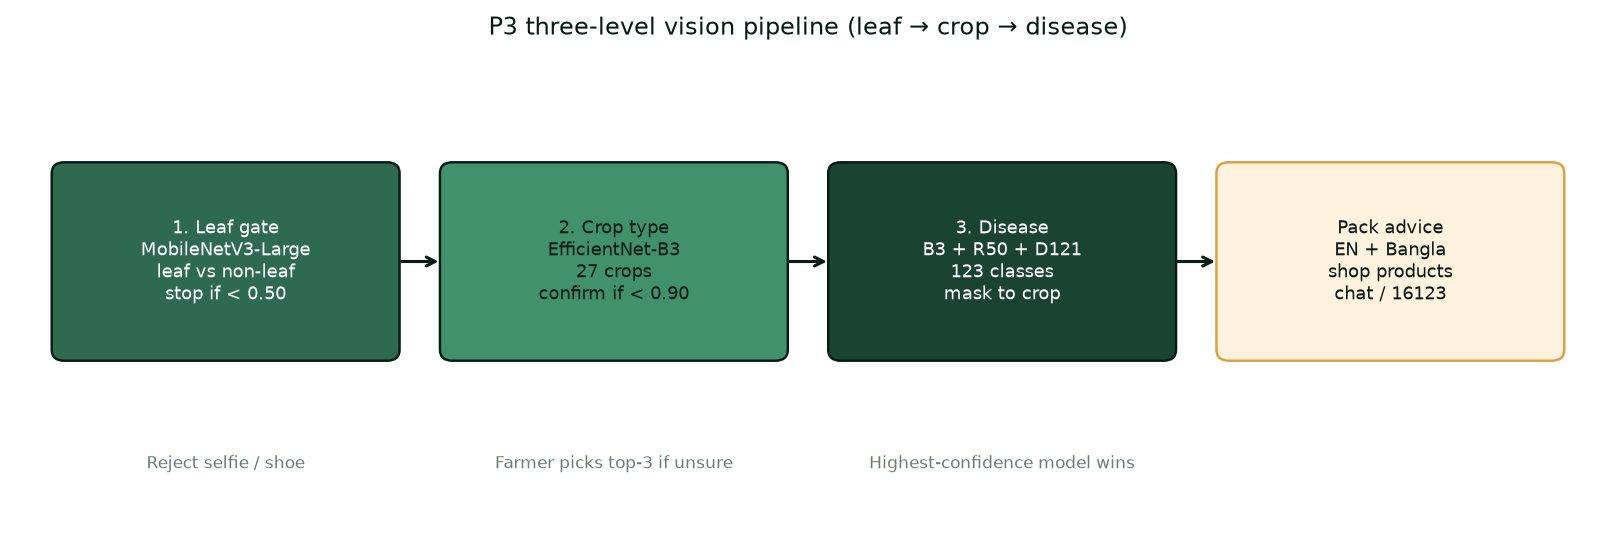
\includegraphics[width=\textwidth]{fig_pipeline.png}
\caption{Leaf gate, crop, disease, then pack advice.}
\end{figure}

\begin{figure}[H]
\centering
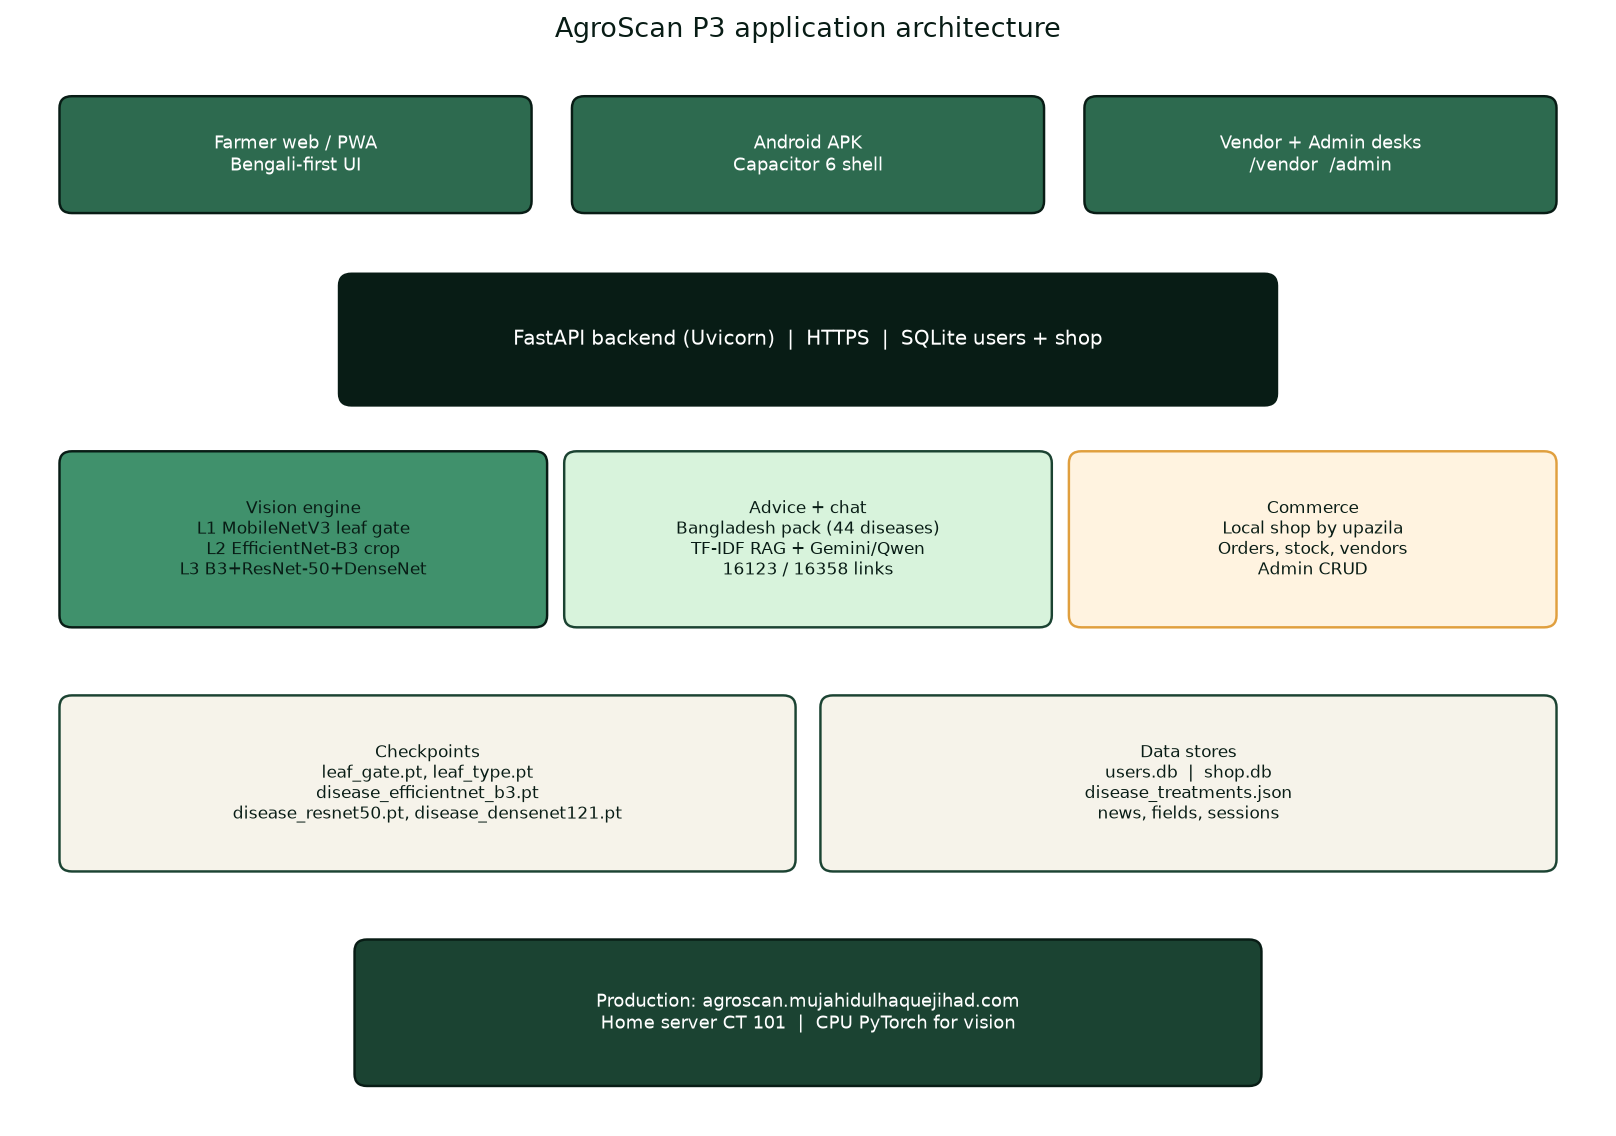
\includegraphics[width=\textwidth]{fig_architecture.png}
\caption{Web / APK / vendor / admin all hit the same FastAPI process.}
\end{figure}

\chapter{Vision pipeline (say this slowly)}
\section{Level 1 --- leaf gate}
File: \texttt{agroscan/infer.py}. Model file: \texttt{models/leaf\_gate.pt}. Architecture: MobileNetV3-Large. Size $224\times224$. Classes: \texttt{leaf}, \texttt{non\_leaf}. Threshold \texttt{LEAF\_ACCEPT\_THRESHOLD = 0.5} in \texttt{agroscan/config.py} line 162.

\texttt{\_leaf\_stage} (187--211) runs softmax, finds the leaf index, returns \texttt{is\_leaf}. If false, \texttt{predict} returns immediately with a Bangla message (409--413). \textbf{Why:} a disease net always picks \emph{some} class. A selfie would become ``tomato blight'' without the gate.

\section{Level 2 --- crop}
File: same. Checkpoint: \texttt{models/leaf\_type.pt}. EfficientNet-B3. Size $300\times300$. 27 crops. \texttt{\_crop\_stage} (225--278). If confidence $<$ \texttt{CROP\_USER\_CONFIRM\_THRESHOLD} (0.90, config line 164), \texttt{needs\_user\_pick} is set and disease is skipped (445--455). If the crop looks like ``Other'' (\texttt{CROP\_OTHER\_THRESHOLD} 0.55), disease is skipped.

\textbf{Why crop first:} tomato early blight and potato early blight are different pack cards. Masking happens in \texttt{\_mask\_probs}.

\section{Level 3 --- disease ensemble}
Three checkpoints from \texttt{config.DISEASE\_ARCHS}: EfficientNet-B3, ResNet-50, DenseNet-121. About 123 classes named \texttt{Crop\_\_\_Disease}. Each model softmax is aligned onto the largest vocabulary (\texttt{\_align\_probs}, 157--165). Then each vector is masked to the chosen crop. \textbf{We do not average.} Line 341: \texttt{winner = max(per\_model, key=confidence)}. That is the sentence they want.

Flags on the winner: \texttt{uncertain} if conf $< 0.45$, \texttt{low\_confidence} if conf $< 0.80$ (\texttt{config.py} 158--160). Advice is attached via \texttt{advice\_for} (380--382).

\texttt{\_pretty} (70--91) splits \texttt{Tomato\_\_\_Late\_blight} into plant + condition.

\section{Preprocessing}
\texttt{agroscan/image\_io.py} \texttt{load\_rgb\_image} turns bytes/PIL into RGB. Optional auto-crop: \texttt{agroscan/leaf\_crop.py} \texttt{auto\_crop\_leaf} (HSV green mask + largest contour), exposed as \texttt{POST /api/preprocess/auto-crop}. Transforms: \texttt{agroscan/data.py} \texttt{infer\_transform}.

\chapter{Training and data}
Command: \texttt{python -m agroscan.train\_all} $\rightarrow$ \texttt{train\_leaf.py}, \texttt{train\_crop.py}, \texttt{train\_disease.py}. Shared loop: \texttt{engine.train\_model}. Loss: \texttt{FocalLoss} (engine.py 18--33) if \texttt{USE\_FOCAL\_LOSS}. Checkpoints: \texttt{models/leaf\_gate.pt}, \texttt{leaf\_type.pt}, \texttt{disease\_efficientnet\_b3.pt}, \texttt{disease\_resnet50.pt}, \texttt{disease\_densenet121.pt}. Resume files: \texttt{*.train.pt}.

Folders: \texttt{Datasets/leaf\_gate/}, \texttt{Datasets/leaf\_type/}, \texttt{Datasets/train|valid|test/}. Sources: PlantVillage, PlantDoc, Bangladesh sets. \texttt{data.py} \texttt{disease\_loaders} / \texttt{combined\_disease\_loaders} build the DataLoaders.

\textbf{If they ask why accuracy is high:} large test set ($\sim$30k images), transfer learning, three similar CNNs. \textbf{Honest limit:} test photos are still cleaner than a dark field phone photo. That is why the gate and the 90\% crop confirm exist.

\chapter{Advice, chat, RAG}
\section{Pack}
\texttt{data/agroscan/} JSON cards (about 44 diseases, EN+BN). \texttt{knowledge.py} \texttt{advice\_for} maps a vision class name onto a card (pathogen, symptoms, cultural control, chemicals, 16123). Chat formatting: \texttt{\_format\_pack\_reply} (599). Name matching: \texttt{resolve\_disease\_query} (803).

\section{Chat order (memorise)}
\texttt{llm\_chat.chat\_reply} (932--1026):
\begin{enumerate}
    \item Clarify if the name fits several crops (\texttt{source: clarify}).
    \item Pack catalog / matched pack (\texttt{source: pack}) --- LLM is not called.
    \item Small KB: hello, 16123, how to use the app (\texttt{knowledge.chatbot\_reply}, 888).
    \item If Gemini is on: \texttt{generate\_reply} with RAG snippets (\texttt{source: gemini+rag}).
    \item Else optional local Qwen. If the text looks bad, fall back to KB.
\end{enumerate}

\section{RAG}
Not FAISS. Sklearn TF-IDF + cosine in \texttt{agroscan/rag.py} \texttt{retrieve}. Top 6 chunks. If a disease key is already known, \texttt{allow\_keys} pins retrieval so rice blast pages cannot leak maize blight doses.

HTTP: \texttt{POST /api/chat} $\rightarrow$ \texttt{backend/main.py} \texttt{chat} (265). Vision+chat wrap: \texttt{POST /api/chat/vision} $\rightarrow$ \texttt{vision\_scan\_reply} (1166).

\chapter{Shop, vendor, admin, accounts}
SQLite \texttt{shop.db}. Schema and queries: \texttt{agroscan/shop\_db.py}. Seed from pack: \texttt{shop\_seed.py} \texttt{seed\_from\_pack}, called at API startup if the catalogue is thin.

Farmer: \texttt{GET /api/shop/products}, \texttt{POST /api/shop/orders}. Vendor token $\neq$ farmer token $\neq$ admin token. Vendor may only see their \texttt{supplier\_id} orders (\texttt{vendor\_order\_detail}, main.py 1028). Vendor shop profile: \texttt{PATCH /api/vendor/me} (982). Farmer auth: \texttt{auth\_store.py} + \texttt{/api/auth/*}.

\chapter{Frontend files (what each JS file is for)}
\begin{itemize}
    \item \texttt{config.js} --- \texttt{API\_BASE}, online pill against \texttt{/api/status}.
    \item \texttt{i18n.js} --- Bangla/English strings.
    \item \texttt{core.js} --- status, upload, analyze, render diagnosis.
    \item \texttt{app-extra.js} --- chat panel, mic, speech, vision-in-chat.
    \item \texttt{shop.js} --- catalogue, cart, checkout, orders.
    \item \texttt{field.js} --- named plots.
    \item \texttt{auth.js} / \texttt{account.js} --- login header and account page.
    \item \texttt{crop.js} --- perspective / auto-crop UI.
    \item \texttt{ops.js} --- shared helpers for vendor/admin HTML.
    \item Vendor UI lives in \texttt{web/vendor.html} (inline script). Admin in \texttt{web/admin.html}.
    \item Android: \texttt{mobile/} Capacitor shell. No on-device ensemble.
\end{itemize}

\chapter{API list you should be able to name}
Diagnosis: \texttt{GET /api/status}, \texttt{POST /api/predict}, \texttt{POST /api/preprocess/auto-crop}. Chat: \texttt{POST /api/chat}, \texttt{POST /api/chat/vision}, \texttt{POST /api/chat/stt}. Shop: \texttt{/api/shop/products}, \texttt{/api/shop/orders}. Auth: \texttt{/api/auth/signup|login|me}. Vendor: \texttt{/api/vendor/login}, \texttt{/me}, \texttt{/orders}, \texttt{/listings}. Admin: \texttt{/api/admin/login}, users, orders, products, vendors. HTML pages: \texttt{/}, \texttt{/vendor}, \texttt{/admin}. Every route function is in Table~\ref{tab:pyapi}.

\chapter{Likely viva questions}
\begin{enumerate}
    \item \textbf{Why three levels?} Disease nets always output a class. Gate stops non-leaves. Crop locking stops tomato spots being called rice blast.
    \item \textbf{Why not average the three disease models?} A weak model would dilute a confident one. Code takes the max confidence (infer.py 341).
    \item \textbf{Why is advice not from the CNN?} CNNs see pixels. Doses and 16123 come from a curated pack (\texttt{advice\_for}).
    \item \textbf{What if crop confidence is 70\%?} Farmer must pick from top-3. Disease does not run yet.
    \item \textbf{Bengali?} Default UI language. Pack and chat have BN strings. \texttt{i18n.js}.
    \item \textbf{Can it work offline?} Shell/PWA cache the UI. Diagnosis needs the server. ONNX was removed from the APK.
    \item \textbf{Animal disease?} In the literature, not in the running app. Say that clearly.
    \item \textbf{Grad-CAM?} Used in the model-comparison notebook, not on every farmer card. Trust in production is gate + crop confirm + pack + helpline.
    \item \textbf{Imbalance?} Focal loss + balanced sampler in \texttt{engine.py} / \texttt{data.py}.
    \item \textbf{Security?} Separate tokens; vendor scoped to supplier; hashed passwords; no mixing farmer and admin sessions.
\end{enumerate}

\chapter{Python function index}
Open the file at the line in the right-hand column. Nested helpers inside a function are not listed; only top-level functions and class methods.

\begin{center}
\footnotesize
\begin{longtable}{@{}p{4.6cm}p{5.2cm}c@{}}
\caption{Vision engine, training loop, and image helpers.}\\
\label{tab:pyvis}\\
\toprule
\textbf{File} & \textbf{Function} & \textbf{Lines} \\
\midrule
\endfirsthead
\toprule
\textbf{File} & \textbf{Function} & \textbf{Lines} \\
\midrule
\endhead
agroscan/config.py & \_split\_has\_classes & 54--55 \\
agroscan/config.py & disease\_ckpt & 106--107 \\
agroscan/config.py & model\_display\_name & 178--179 \\
agroscan/config.py & load\_dotenv & 182--199 \\
agroscan/data.py & \_folder\_image\_loader & 26--28 \\
agroscan/data.py & build\_transforms & 34--54 \\
agroscan/data.py & infer\_transform & 57--58 \\
agroscan/data.py & \_dataloader\_kwargs & 61--72 \\
agroscan/data.py & ImageListDataset.\_\_init\_\_ & 79--81 \\
agroscan/data.py & ImageListDataset.\_\_len\_\_ & 83--84 \\
agroscan/data.py & ImageListDataset.\_\_getitem\_\_ & 86--89 \\
agroscan/data.py & \_gather & 92--93 \\
agroscan/data.py & \_class\_image\_paths & 96--106 \\
agroscan/data.py & \_stratified\_split & 109--126 \\
agroscan/data.py & \_items\_from\_imagefolder\_root & 129--137 \\
agroscan/data.py & \_plantvillage\_class\_names & 140--145 \\
agroscan/data.py & \_plantvillage\_only\_loaders & 151--167 \\
agroscan/data.py & \_combined\_disease\_items & 170--252 \\
agroscan/data.py & DiseaseImageFolder.\_\_init\_\_ & 258--265 \\
agroscan/data.py & DiseaseImageFolder.find\_classes & 268--280 \\
agroscan/data.py & class\_weights\_for\_dataset & 283--290 \\
agroscan/data.py & \_make\_loader & 293--305 \\
agroscan/data.py & \_unified\_split\_loaders & 308--320 \\
agroscan/data.py & crop\_loaders & 323--337 \\
agroscan/data.py & combined\_disease\_loaders & 340--367 \\
agroscan/data.py & disease\_loaders & 370--399 \\
agroscan/data.py & disease\_image\_paths\_for\_leaf\_gate & 402--443 \\
agroscan/data.py & \_leaf\_items & 449--473 \\
agroscan/data.py & leaf\_loaders & 476--516 \\
agroscan/engine.py & FocalLoss.\_\_init\_\_ & 21--27 \\
agroscan/engine.py & FocalLoss.forward & 29--33 \\
agroscan/engine.py & evaluate & 37--45 \\
agroscan/engine.py & train\_resume\_path & 48--50 \\
agroscan/engine.py & train\_model & 53--188 \\
agroscan/image\_io.py & openable\_path & 12--19 \\
agroscan/image\_io.py & \_downscale\_if\_needed & 72--79 \\
agroscan/image\_io.py & \_to\_rgb & 82--96 \\
agroscan/image\_io.py & load\_rgb\_image & 99--139 \\
agroscan/image\_io.py & sniff\_image\_path & 142--157 \\
agroscan/image\_io.py & is\_image\_path & 160--168 \\
agroscan/image\_io.py & gather\_images & 171--179 \\
agroscan/infer.py & \_ensure\_other\_option & 27--32 \\
agroscan/infer.py & \_decorate\_crop & 35--53 \\
agroscan/infer.py & \_other\_crop\_message & 56--67 \\
agroscan/infer.py & \_pretty & 70--91 \\
agroscan/infer.py & LoadedModel.\_\_init\_\_ & 95--100 \\
agroscan/infer.py & LoadedModel.probs & 103--105 \\
agroscan/infer.py & InferenceEngine.\_\_init\_\_ & 109--134 \\
agroscan/infer.py & InferenceEngine.ready & 138--139 \\
agroscan/infer.py & InferenceEngine.status & 141--154 \\
agroscan/infer.py & InferenceEngine.\_align\_probs & 157--165 \\
agroscan/infer.py & InferenceEngine.\_disease\_prob\_stack & 167--185 \\
agroscan/infer.py & InferenceEngine.\_leaf\_stage & 187--211 \\
agroscan/infer.py & InferenceEngine.\_top\_crops\_from\_probs & 213--223 \\
agroscan/infer.py & InferenceEngine.\_crop\_stage & 225--278 \\
agroscan/infer.py & InferenceEngine.\_mask\_probs & 280--290 \\
agroscan/infer.py & InferenceEngine.\_disease\_stage & 292--389 \\
agroscan/infer.py & InferenceEngine.predict & 392--472 \\
agroscan/label\_map.py & merge\_class\_name & 73--76 \\
agroscan/label\_map.py & is\_variety\_class & 79--80 \\
agroscan/label\_map.py & is\_other\_crop & 83--85 \\
agroscan/label\_map.py & crop\_from\_class & 88--103 \\
agroscan/label\_map.py & classes\_for\_crop & 106--114 \\
agroscan/label\_map.py & merge\_key & 117--135 \\
agroscan/label\_map.py & \_bd\_to\_canonical & 138--148 \\
agroscan/label\_map.py & \_mango\_variety\_to\_canonical & 151--155 \\
agroscan/label\_map.py & \_bd\_leaf\_to\_canonical & 158--163 \\
agroscan/label\_map.py & canonical\_name & 166--201 \\
agroscan/label\_map.py & LabelRegistry.\_\_init\_\_ & 207--211 \\
agroscan/label\_map.py & LabelRegistry.class\_names & 214--215 \\
agroscan/label\_map.py & LabelRegistry.register & 217--225 \\
agroscan/label\_map.py & LabelRegistry.label\_for & 227--228 \\
agroscan/label\_map.py & summarize\_registry & 231--238 \\
agroscan/land\_scale.py & to\_decimals & 8--23 \\
agroscan/land\_scale.py & \_first\_range & 26--41 \\
agroscan/land\_scale.py & water\_litres\_per\_decimal & 44--55 \\
agroscan/land\_scale.py & dose\_per\_litre & 58--112 \\
agroscan/land\_scale.py & kg\_per\_bigha & 115--143 \\
agroscan/land\_scale.py & land\_band & 146--153 \\
agroscan/land\_scale.py & followup\_steps & 156--241 \\
agroscan/land\_scale.py & scale\_chemical & 244--317 \\
agroscan/land\_scale.py & scale\_fertilizer\_note & 320--338 \\
agroscan/land\_scale.py & land\_summary & 341--354 \\
agroscan/leaf\_crop.py & \_pil\_to\_bgr & 20--22 \\
agroscan/leaf\_crop.py & \_bgr\_to\_pil & 25--27 \\
agroscan/leaf\_crop.py & \_leaf\_mask & 30--60 \\
agroscan/leaf\_crop.py & \_largest\_contour & 63--67 \\
agroscan/leaf\_crop.py & auto\_crop\_leaf & 76--144 \\
agroscan/leaf\_crop.py & perspective\_crop & 147--175 \\
agroscan/leaf\_crop.py & image\_to\_jpeg\_bytes & 178--181 \\
agroscan/models.py & build\_model & 11--41 \\
agroscan/models.py & save\_checkpoint & 44--53 \\
agroscan/models.py & save\_training\_state & 56--58 \\
agroscan/models.py & load\_training\_state & 61--67 \\
agroscan/models.py & load\_checkpoint & 70--80 \\
\bottomrule
\end{longtable}
\end{center}
\begin{center}
\footnotesize
\begin{longtable}{@{}p{4.6cm}p{5.2cm}c@{}}
\caption{Chat, pack, RAG, and advice.}\\
\label{tab:pychat}\\
\toprule
\textbf{File} & \textbf{Function} & \textbf{Lines} \\
\midrule
\endfirsthead
\toprule
\textbf{File} & \textbf{Function} & \textbf{Lines} \\
\midrule
\endhead
agroscan/farm\_plan.py & season\_for\_month & 22--27 \\
agroscan/farm\_plan.py & load\_flora\_crops & 75--94 \\
agroscan/farm\_plan.py & load\_csv\_crop\_rows & 98--116 \\
agroscan/farm\_plan.py & \_land\_note & 119--138 \\
agroscan/farm\_plan.py & recommend\_crops & 141--299 \\
agroscan/farm\_plan.py & cultivation\_outline & 302--370 \\
agroscan/knowledge.py & \_attach\_guide & 297--309 \\
agroscan/knowledge.py & \_localize\_info & 312--326 \\
agroscan/knowledge.py & advice\_for\_key & 329--362 \\
agroscan/knowledge.py & advice\_for & 365--386 \\
agroscan/knowledge.py & all\_diseases & 389--409 \\
agroscan/knowledge.py & \_contacts\_text & 422--430 \\
agroscan/knowledge.py & \_is\_healthy\_rec & 469--472 \\
agroscan/knowledge.py & wants\_catalog & 475--485 \\
agroscan/knowledge.py & \_catalog\_reply\_lang & 488--496 \\
agroscan/knowledge.py & pack\_catalog\_reply & 499--575 \\
agroscan/knowledge.py & \_split\_name & 578--579 \\
agroscan/knowledge.py & \_disease\_name\_tokens & 582--596 \\
agroscan/knowledge.py & \_format\_pack\_reply & 599--634 \\
agroscan/knowledge.py & \_option\_label & 637--642 \\
agroscan/knowledge.py & \_score\_pack\_candidates & 645--725 \\
agroscan/knowledge.py & \_score\_kb\_candidates & 728--771 \\
agroscan/knowledge.py & \_clarify\_payload & 774--800 \\
agroscan/knowledge.py & resolve\_disease\_query & 803--867 \\
agroscan/knowledge.py & resolve\_disease\_advice & 870--879 \\
agroscan/knowledge.py & \_suggestions & 882--885 \\
agroscan/knowledge.py & chatbot\_reply & 888--1014 \\
agroscan/llm\_chat.py & \_env\_flag & 63--64 \\
agroscan/llm\_chat.py & \_adapter\_path & 67--74 \\
agroscan/llm\_chat.py & \_gemini\_key & 77--81 \\
agroscan/llm\_chat.py & \_gemini\_enabled & 84--88 \\
agroscan/llm\_chat.py & \_want\_local\_llm & 91--92 \\
agroscan/llm\_chat.py & \_local\_base\_id & 95--96 \\
agroscan/llm\_chat.py & \_local\_provider & 99--105 \\
agroscan/llm\_chat.py & llm\_configured & 108--123 \\
agroscan/llm\_chat.py & llm\_status & 126--146 \\
agroscan/llm\_chat.py & \_structural\_intent & 149--170 \\
agroscan/llm\_chat.py & \_kb\_is\_generic & 173--177 \\
agroscan/llm\_chat.py & \_relevant\_context & 180--215 \\
agroscan/llm\_chat.py & \_sanitize\_history & 231--255 \\
agroscan/llm\_chat.py & \_pack\_keys & 258--265 \\
agroscan/llm\_chat.py & \_llm\_looks\_unsure & 268--314 \\
agroscan/llm\_chat.py & \_gemini\_contents & 317--336 \\
agroscan/llm\_chat.py & \_reply\_lang & 339--353 \\
agroscan/llm\_chat.py & \_build\_chat\_messages & 356--469 \\
agroscan/llm\_chat.py & \_fold\_system\_into\_user & 472--484 \\
agroscan/llm\_chat.py & \_to\_chat\_prompt & 487--498 \\
agroscan/llm\_chat.py & \_resolve\_device & 501--509 \\
agroscan/llm\_chat.py & \_want\_4bit & 512--518 \\
agroscan/llm\_chat.py & \_load\_base & 521--558 \\
agroscan/llm\_chat.py & \_ensure\_loaded & 561--638 \\
agroscan/llm\_chat.py & preload & 641--651 \\
agroscan/llm\_chat.py & \_generate\_text & 654--681 \\
agroscan/llm\_chat.py & \_gemini\_models & 684--693 \\
agroscan/llm\_chat.py & \_gemini\_extract\_text & 696--698 \\
agroscan/llm\_chat.py & \_gemini\_extract & 701--709 \\
agroscan/llm\_chat.py & \_gemini\_http & 712--725 \\
agroscan/llm\_chat.py & \_gemini\_generate & 728--813 \\
agroscan/llm\_chat.py & generate\_reply & 816--836 \\
agroscan/llm\_chat.py & transcribe\_audio & 842--929 \\
agroscan/llm\_chat.py & chat\_reply & 932--1026 \\
agroscan/llm\_chat.py & \_scan\_header & 1029--1046 \\
agroscan/llm\_chat.py & \_build\_vision\_messages & 1049--1108 \\
agroscan/llm\_chat.py & \_llm\_text\_is\_bad & 1111--1137 \\
agroscan/llm\_chat.py & generate\_vision\_feedback & 1140--1163 \\
agroscan/llm\_chat.py & vision\_scan\_reply & 1166--1310 \\
agroscan/news.py & \_load\_raw & 14--21 \\
agroscan/news.py & \_pick & 24--28 \\
agroscan/news.py & \_seasonal\_extra & 31--70 \\
agroscan/news.py & list\_news & 73--127 \\
agroscan/rag.py & \_section\_bodies & 29--64 \\
agroscan/rag.py & \_guide\_text & 67--78 \\
agroscan/rag.py & \_info\_text & 81--90 \\
agroscan/rag.py & \_load\_pack\_docs & 93--109 \\
agroscan/rag.py & \_pack\_chunks & 112--141 \\
agroscan/rag.py & \_legacy\_chunks & 144--167 \\
agroscan/rag.py & \_chunks & 170--176 \\
agroscan/rag.py & clear\_index\_cache & 179--180 \\
agroscan/rag.py & \_index & 184--193 \\
agroscan/rag.py & \_key\_ok & 196--218 \\
agroscan/rag.py & \_section\_boost & 221--232 \\
agroscan/rag.py & retrieve & 235--289 \\
agroscan/rag\_build.py & \_is\_healthy & 19--22 \\
agroscan/rag\_build.py & \_lines & 25--48 \\
agroscan/rag\_build.py & \_chem\_block & 51--98 \\
agroscan/rag\_build.py & \_pick & 101--104 \\
agroscan/rag\_build.py & build\_disease\_doc & 107--230 \\
agroscan/rag\_build.py & build\_all & 233--251 \\
agroscan/treatment\_detail.py & \_pick & 21--24 \\
agroscan/treatment\_detail.py & \_warnings\_for & 27--81 \\
agroscan/treatment\_detail.py & \_chem\_display & 84--111 \\
agroscan/treatment\_detail.py & treatment\_plan\_for & 114--124 \\
agroscan/treatment\_detail.py & \_plan\_from\_record & 127--164 \\
agroscan/treatment\_detail.py & advice\_from\_pack & 167--238 \\
\bottomrule
\end{longtable}
\end{center}
\begin{center}
\footnotesize
\begin{longtable}{@{}p{4.6cm}p{5.2cm}c@{}}
\caption{Shop database and farmer authentication.}\\
\label{tab:pyshop}\\
\toprule
\textbf{File} & \textbf{Function} & \textbf{Lines} \\
\midrule
\endfirsthead
\toprule
\textbf{File} & \textbf{Function} & \textbf{Lines} \\
\midrule
\endhead
agroscan/auth\_store.py & \_connect & 16--20 \\
agroscan/auth\_store.py & \_ensure\_delivery\_columns & 23--36 \\
agroscan/auth\_store.py & init\_db & 39--63 \\
agroscan/auth\_store.py & \_hash\_password & 66--69 \\
agroscan/auth\_store.py & \_check\_password & 72--78 \\
agroscan/auth\_store.py & \_user\_dict & 81--101 \\
agroscan/auth\_store.py & \_session\_counts & 104--117 \\
agroscan/auth\_store.py & \_new\_token & 120--121 \\
agroscan/auth\_store.py & \_expires\_at & 124--125 \\
agroscan/auth\_store.py & create\_local\_user & 128--165 \\
agroscan/auth\_store.py & login\_local & 168--178 \\
agroscan/auth\_store.py & get\_user\_by\_token & 181--198 \\
agroscan/auth\_store.py & upsert\_google\_user & 201--220 \\
agroscan/auth\_store.py & create\_session & 223--231 \\
agroscan/auth\_store.py & delete\_session & 234--239 \\
agroscan/auth\_store.py & update\_user\_profile & 242--278 \\
agroscan/auth\_store.py & admin\_list\_users & 281--303 \\
agroscan/auth\_store.py & admin\_get\_user & 306--313 \\
agroscan/auth\_store.py & admin\_update\_user & 316--399 \\
agroscan/auth\_store.py & admin\_revoke\_user\_sessions & 402--407 \\
agroscan/auth\_store.py & admin\_delete\_user & 410--418 \\
agroscan/auth\_store.py & admin\_user\_stats & 421--444 \\
agroscan/shop\_db.py & \_connect & 28--33 \\
agroscan/shop\_db.py & init\_shop\_db & 36--164 \\
agroscan/shop\_db.py & \_ensure\_columns & 167--205 \\
agroscan/shop\_db.py & product\_price & 208--223 \\
agroscan/shop\_db.py & update\_product\_price & 226--243 \\
agroscan/shop\_db.py & list\_products\_admin & 246--247 \\
agroscan/shop\_db.py & \_now & 250--251 \\
agroscan/shop\_db.py & \_row\_dict & 254--255 \\
agroscan/shop\_db.py & list\_upazilas & 258--290 \\
agroscan/shop\_db.py & \_enrich\_upazila\_bn & 293--319 \\
agroscan/shop\_db.py & \_haversine\_km & 321--328 \\
agroscan/shop\_db.py & nearest\_upazila & 331--351 \\
agroscan/shop\_db.py & list\_suppliers & 354--392 \\
agroscan/shop\_db.py & list\_products & 395--436 \\
agroscan/shop\_db.py & product\_with\_suppliers & 439--460 \\
agroscan/shop\_db.py & recommended\_products\_for\_disease & 463--522 \\
agroscan/shop\_db.py & \_order\_code & 525--526 \\
agroscan/shop\_db.py & create\_order & 529--617 \\
agroscan/shop\_db.py & get\_order & 620--644 \\
agroscan/shop\_db.py & list\_orders & 647--685 \\
agroscan/shop\_db.py & admin\_shop\_stats & 688--717 \\
agroscan/shop\_db.py & update\_order\_status & 720--747 \\
agroscan/shop\_db.py & update\_order & 750--839 \\
agroscan/shop\_db.py & pick\_supplier\_id & 842--853 \\
agroscan/shop\_db.py & assign\_order\_supplier & 856--873 \\
agroscan/shop\_db.py & list\_suppliers\_admin & 876--900 \\
agroscan/shop\_db.py & get\_supplier & 903--908 \\
agroscan/shop\_db.py & list\_supplier\_listings & 911--943 \\
agroscan/shop\_db.py & update\_supplier\_listing & 946--986 \\
agroscan/shop\_db.py & upsert\_supplier\_listing & 989--1022 \\
agroscan/shop\_db.py & update\_supplier\_profile & 1025--1041 \\
agroscan/shop\_db.py & vendor\_self\_update & 1044--1068 \\
agroscan/shop\_db.py & \_vendor\_username & 1071--1075 \\
agroscan/shop\_db.py & \_vendor\_dict & 1078--1092 \\
agroscan/shop\_db.py & \_ensure\_default\_vendor & 1095--1141 \\
agroscan/shop\_db.py & list\_vendors & 1144--1162 \\
agroscan/shop\_db.py & create\_vendor & 1165--1184 \\
agroscan/shop\_db.py & reset\_vendor\_password & 1187--1201 \\
agroscan/shop\_db.py & update\_vendor & 1204--1245 \\
agroscan/shop\_db.py & set\_vendor\_active & 1248--1258 \\
agroscan/shop\_db.py & vendor\_login & 1261--1282 \\
agroscan/shop\_db.py & vendor\_logout & 1285--1289 \\
agroscan/shop\_db.py & get\_vendor\_by\_token & 1292--1315 \\
agroscan/shop\_db.py & vendor\_stats & 1318--1354 \\
agroscan/shop\_seed.py & \_product\_image\_map & 14--22 \\
agroscan/shop\_seed.py & \_short\_desc\_map & 25--33 \\
agroscan/shop\_seed.py & \_image\_url\_for & 36--41 \\
agroscan/shop\_seed.py & \_short\_description & 44--63 \\
agroscan/shop\_seed.py & seed\_from\_pack & 66--255 \\
agroscan/shop\_seed.py & apply\_product\_images & 258--298 \\
\bottomrule
\end{longtable}
\end{center}
\begin{center}
\footnotesize
\begin{longtable}{@{}p{4.6cm}p{5.2cm}c@{}}
\caption{FastAPI routes and helpers in backend/main.py.}\\
\label{tab:pyapi}\\
\toprule
\textbf{File} & \textbf{Function} & \textbf{Lines} \\
\midrule
\endfirsthead
\toprule
\textbf{File} & \textbf{Function} & \textbf{Lines} \\
\midrule
\endhead
backend/main.py & \_optional\_user & 95--98 \\
backend/main.py & \_load & 102--123 \\
backend/main.py & status & 127--133 \\
backend/main.py & llm\_load & 137--144 \\
backend/main.py & classes & 148--149 \\
backend/main.py & predict & 153--182 \\
backend/main.py & preprocess\_auto\_crop & 190--206 \\
backend/main.py & preprocess\_perspective\_crop & 210--225 \\
backend/main.py & chat\_stt & 249--262 \\
backend/main.py & chat & 266--286 \\
backend/main.py & chat\_vision & 290--322 \\
backend/main.py & resources & 326--327 \\
backend/main.py & news & 331--333 \\
backend/main.py & advice & 337--352 \\
backend/main.py & diseases & 356--359 \\
backend/main.py & crops\_catalog & 375--378 \\
backend/main.py & farm\_plan & 382--395 \\
backend/main.py & farm\_cultivate & 399--402 \\
backend/main.py & shop\_upazilas & 483--484 \\
backend/main.py & shop\_nearest\_upazila & 488--492 \\
backend/main.py & shop\_suppliers & 496--507 \\
backend/main.py & shop\_products & 511--521 \\
backend/main.py & shop\_product & 525--529 \\
backend/main.py & shop\_recommend & 533--534 \\
backend/main.py & shop\_create\_order & 538--555 \\
backend/main.py & shop\_orders & 559--562 \\
backend/main.py & shop\_order\_detail & 566--573 \\
backend/main.py & \_admin\_expected\_token & 579--580 \\
backend/main.py & \_admin\_expected\_user & 583--584 \\
backend/main.py & \_admin\_token\_ok & 587--593 \\
backend/main.py & \_vendor\_user & 596--602 \\
backend/main.py & admin\_login & 606--611 \\
backend/main.py & admin\_orders & 615--627 \\
backend/main.py & admin\_order\_detail & 631--637 \\
backend/main.py & admin\_stats & 641--656 \\
backend/main.py & admin\_users & 660--668 \\
backend/main.py & admin\_user\_detail & 672--678 \\
backend/main.py & admin\_user\_update & 693--714 \\
backend/main.py & admin\_user\_create & 718--738 \\
backend/main.py & admin\_user\_revoke & 742--746 \\
backend/main.py & admin\_user\_delete & 750--757 \\
backend/main.py & admin\_update\_order & 761--797 \\
backend/main.py & admin\_create\_order & 801--823 \\
backend/main.py & admin\_seed & 827--832 \\
backend/main.py & admin\_apply\_images & 836--841 \\
backend/main.py & admin\_products & 844--857 \\
backend/main.py & \_apply\_admin\_product\_price & 860--864 \\
backend/main.py & admin\_set\_product\_price & 868--877 \\
backend/main.py & admin\_update\_product\_price & 881--908 \\
backend/main.py & admin\_suppliers & 912--920 \\
backend/main.py & admin\_vendors\_list & 924--927 \\
backend/main.py & admin\_vendors\_create & 931--938 \\
backend/main.py & admin\_vendors\_patch & 942--959 \\
backend/main.py & vendor\_login\_api & 963--967 \\
backend/main.py & vendor\_logout\_api & 971--974 \\
backend/main.py & vendor\_me & 978--979 \\
backend/main.py & vendor\_me\_patch & 983--1003 \\
backend/main.py & vendor\_stats\_api & 1007--1008 \\
backend/main.py & vendor\_orders\_api & 1012--1024 \\
backend/main.py & vendor\_order\_detail & 1028--1035 \\
backend/main.py & vendor\_update\_order & 1039--1052 \\
backend/main.py & vendor\_listings & 1056--1069 \\
backend/main.py & vendor\_listing\_create & 1073--1083 \\
backend/main.py & vendor\_listing\_patch & 1087--1097 \\
backend/main.py & safety\_ref & 1101--1111 \\
backend/main.py & \_auth\_response & 1137--1139 \\
backend/main.py & auth\_signup & 1143--1158 \\
backend/main.py & auth\_login & 1162--1167 \\
backend/main.py & auth\_logout & 1171--1174 \\
backend/main.py & auth\_me & 1178--1181 \\
backend/main.py & auth\_profile & 1193--1207 \\
backend/main.py & auth\_google & 1211--1232 \\
\bottomrule
\end{longtable}
\end{center}
\begin{center}
\footnotesize
\begin{longtable}{@{}p{4.6cm}p{5.2cm}c@{}}
\caption{Training entrypoints, dataset prep, and helper scripts.}\\
\label{tab:pyrest}\\
\toprule
\textbf{File} & \textbf{Function} & \textbf{Lines} \\
\midrule
\endfirsthead
\toprule
\textbf{File} & \textbf{Function} & \textbf{Lines} \\
\midrule
\endhead
agroscan/bd\_data.py & \_read & 12--16 \\
agroscan/bd\_data.py & treatments & 20--22 \\
agroscan/bd\_data.py & treatments\_by\_class & 26--27 \\
agroscan/bd\_data.py & treatments\_by\_kb & 31--38 \\
agroscan/bd\_data.py & products & 42--44 \\
agroscan/bd\_data.py & equipment & 48--50 \\
agroscan/bd\_data.py & catalogue\_by\_sku & 54--60 \\
agroscan/bd\_data.py & suppliers & 64--66 \\
agroscan/bd\_data.py & upazilas & 70--72 \\
agroscan/bd\_data.py & crops & 76--78 \\
agroscan/bd\_data.py & safety & 82--84 \\
agroscan/bd\_data.py & warning\_boxes & 88--90 \\
agroscan/bd\_data.py & warning\_box & 93--109 \\
agroscan/bd\_data.py & \_norm & 112--121 \\
agroscan/bd\_data.py & find\_treatment & 124--158 \\
agroscan/bd\_data.py & find\_crop & 161--172 \\
agroscan/bd\_dataset.py & \_require\_datasets & 24--31 \\
agroscan/bd\_dataset.py & hf\_repo\_id & 34--35 \\
agroscan/bd\_dataset.py & hf\_access\_help & 38--45 \\
agroscan/bd\_dataset.py & load\_bd\_splits & 48--68 \\
agroscan/bd\_dataset.py & \_label\_names\_from\_train & 71--77 \\
agroscan/bd\_dataset.py & \_row\_label\_name & 80--83 \\
agroscan/bd\_dataset.py & bd\_label\_names & 86--89 \\
agroscan/bd\_dataset.py & bd\_split\_stats & 92--94 \\
agroscan/bd\_dataset.py & export\_to\_imagefolder & 97--127 \\
agroscan/bd\_dataset.py & \_safe\_class\_dir & 130--132 \\
agroscan/bd\_dataset.py & print\_dataset\_info & 135--148 \\
agroscan/bd\_leaf\_dataset.py & find\_bd\_leaf\_zip & 15--20 \\
agroscan/bd\_leaf\_dataset.py & is\_bd\_leaf\_extracted & 23--30 \\
agroscan/bd\_leaf\_dataset.py & ensure\_bd\_leaf\_extracted & 33--78 \\
agroscan/bd\_leaf\_dataset.py & bd\_leaf\_stats & 81--89 \\
agroscan/disease\_guides.py & guide\_for & 514--515 \\
agroscan/prepare\_bd\_dataset.py & \_write\_manifest & 30--42 \\
agroscan/prepare\_bd\_dataset.py & main & 45--95 \\
agroscan/prepare\_bd\_leaf\_dataset.py & main & 16--44 \\
agroscan/prepare\_hierarchy.py & \_unique\_path & 18--28 \\
agroscan/prepare\_hierarchy.py & \_safe\_name & 31--32 \\
agroscan/prepare\_hierarchy.py & \_hardlink & 35--42 \\
agroscan/prepare\_hierarchy.py & \_iter\_images & 45--48 \\
agroscan/prepare\_hierarchy.py & merge\_duplicate\_labels & 51--80 \\
agroscan/prepare\_hierarchy.py & build\_leaf\_type & 83--107 \\
agroscan/prepare\_hierarchy.py & drop\_variety\_from\_disease & 110--124 \\
agroscan/prepare\_hierarchy.py & relocate\_leaf\_gate & 127--140 \\
agroscan/prepare\_hierarchy.py & main & 143--158 \\
agroscan/train\_all.py & main & 12--43 \\
agroscan/train\_crop.py & train\_crop & 15--44 \\
agroscan/train\_crop.py & main & 47--59 \\
agroscan/train\_disease.py & train\_one & 15--41 \\
agroscan/train\_disease.py & main & 44--57 \\
agroscan/train\_leaf.py & train\_leaf & 15--43 \\
agroscan/train\_leaf.py & main & 46--58 \\
scripts/build\_shop\_images.py & load\_font & 48--60 \\
scripts/build\_shop\_images.py & wrap & 63--82 \\
scripts/build\_shop\_images.py & short\_desc & 85--111 \\
scripts/build\_shop\_images.py & palette\_for & 114--127 \\
scripts/build\_shop\_images.py & draw\_pack & 130--167 \\
scripts/build\_shop\_images.py & render\_card & 170--234 \\
scripts/build\_shop\_images.py & load\_rows & 237--247 \\
scripts/build\_shop\_images.py & main & 250--274 \\
scripts/check\_auto\_crop\_fast.py & main & 12--23 \\
scripts/export\_mobile\_onnx.py & \_slim\_advice & 34--52 \\
scripts/export\_mobile\_onnx.py & \_export\_one & 55--89 \\
scripts/export\_mobile\_onnx.py & main & 92--132 \\
scripts/fetch\_shop\_images.py & \_get & 89--92 \\
scripts/fetch\_shop\_images.py & clean\_name & 95--106 \\
scripts/fetch\_shop\_images.py & primary\_key & 109--119 \\
scripts/fetch\_shop\_images.py & search\_terms & 122--150 \\
scripts/fetch\_shop\_images.py & openverse\_search & 153--172 \\
scripts/fetch\_shop\_images.py & pick\_from\_results & 175--189 \\
scripts/fetch\_shop\_images.py & pick\_image & 195--215 \\
scripts/fetch\_shop\_images.py & download\_image & 218--237 \\
scripts/fetch\_shop\_images.py & load\_catalog & 240--250 \\
scripts/fetch\_shop\_images.py & file\_key & 253--256 \\
scripts/fetch\_shop\_images.py & main & 259--337 \\
scripts/fix\_split\_leakage.py & log & 32--33 \\
scripts/fix\_split\_leakage.py & orig\_name & 36--39 \\
scripts/fix\_split\_leakage.py & pv\_source & 42--49 \\
scripts/fix\_split\_leakage.py & file\_id\_entry & 52--57 \\
scripts/fix\_split\_leakage.py & file\_id & 60--65 \\
scripts/fix\_split\_leakage.py & iter\_images & 68--77 \\
scripts/fix\_split\_leakage.py & class\_counts & 80--93 \\
scripts/fix\_split\_leakage.py & keep\_best\_split & 96--103 \\
scripts/fix\_split\_leakage.py & scan\_leaks & 106--149 \\
scripts/fix\_split\_leakage.py & protect\_last\_train & 152--171 \\
scripts/fix\_split\_leakage.py & inode\_index & 174--188 \\
scripts/fix\_split\_leakage.py & cap\_train & 191--209 \\
scripts/fix\_split\_leakage.py & summarize & 212--222 \\
scripts/fix\_split\_leakage.py & main & 225--296 \\
scripts/make\_app\_icons.py & \_key\_black & 49--61 \\
scripts/make\_app\_icons.py & \_trim & 64--66 \\
scripts/make\_app\_icons.py & \_paste\_centered & 69--82 \\
scripts/make\_app\_icons.py & \_square & 85--89 \\
scripts/make\_app\_icons.py & \_save & 92--95 \\
scripts/make\_app\_icons.py & main & 98--154 \\
scripts/scan\_split\_leakage.py & log & 17--18 \\
scripts/scan\_split\_leakage.py & orig\_name & 21--24 \\
scripts/scan\_split\_leakage.py & pv\_source & 27--35 \\
scripts/scan\_split\_leakage.py & scan\_task & 38--93 \\
scripts/scan\_split\_leakage.py & main & 96--127 \\
scripts/test\_rag\_chunking.py & main & 11--47 \\
scripts/test\_split\_leakage.py & main & 9--27 \\
\bottomrule
\end{longtable}
\end{center}

\chapter{JavaScript function index}
These are \texttt{function name(} declarations inside \texttt{web/*.js}. Vendor and admin logic that sits in the HTML script tags is not in this list; read \texttt{web/vendor.html} and \texttt{web/admin.html} for those desks.

\begin{center}
\footnotesize
\begin{longtable}{@{}p{4.6cm}p{5.2cm}c@{}}
\caption{JavaScript functions in web/*.js.}\\
\label{tab:js}\\
\toprule
\textbf{File} & \textbf{Function} & \textbf{Lines} \\
\midrule
\endfirsthead
\toprule
\textbf{File} & \textbf{Function} & \textbf{Lines} \\
\midrule
\endhead
web/account.js & T & 7 \\
web/account.js & esc & 10 \\
web/account.js & session & 15 \\
web/account.js & token & 18 \\
web/account.js & isRealUser & 22 \\
web/account.js & xhr & 27 \\
web/account.js & fmtWhen & 46 \\
web/account.js & statusLabel & 57 \\
web/account.js & timelineHtml & 63 \\
web/account.js & renderOrderCard & 82 \\
web/account.js & renderDetail & 94 \\
web/account.js & loadOrderDetail & 132 \\
web/account.js & setTab & 144 \\
web/account.js & dash & 157 \\
web/account.js & fillProfile & 165 \\
web/account.js & setEditMode & 191 \\
web/account.js & cancelEdit & 208 \\
web/account.js & saveProfile & 220 \\
web/account.js & loadOrders & 250 \\
web/account.js & showApp & 287 \\
web/account.js & showGate & 304 \\
web/account.js & init & 309 \\
web/ads.js & t & 13 \\
web/ads.js & setStrip & 19 \\
web/ads.js & nextStrip & 40 \\
web/ads.js & startRotate & 45 \\
web/ads.js & stopRotate & 51 \\
web/ads.js & closePopup & 58 \\
web/ads.js & showPopup & 64 \\
web/ads.js & boot & 74 \\
web/app-extra.js & init & 7 \\
web/app-extra.js & i18n & 35 \\
web/app-extra.js & catLabel & 37 \\
web/app-extra.js & visitLabel & 42 \\
web/app-extra.js & esc & 46 \\
web/app-extra.js & renderGovCard & 50 \\
web/app-extra.js & renderEmergencyCard & 65 \\
web/app-extra.js & paintEmergency & 76 \\
web/app-extra.js & filterGovLinks & 84 \\
web/app-extra.js & paintGovGrid & 97 \\
web/app-extra.js & setupGovHub & 107 \\
web/app-extra.js & loadResources & 127 \\
web/app-extra.js & setupDragDrop & 149 \\
web/app-extra.js & setupChat & 164 \\
web/app-extra.js & tChat & 229 \\
web/app-extra.js & isBnChat & 234 \\
web/app-extra.js & chatSourceLabel & 257 \\
web/app-extra.js & rememberChatDisease & 267 \\
web/app-extra.js & pushChatBot & 273 \\
web/app-extra.js & collectChatHistory & 294 \\
web/app-extra.js & pushChatUserImage & 314 \\
web/app-extra.js & postChatVision & 336 \\
web/app-extra.js & chatAnalyzeImage & 370 \\
web/app-extra.js & handleChatVisionResult & 396 \\
web/app-extra.js & refreshMicTitle & 473 \\
web/app-extra.js & refreshSpeakTitle & 482 \\
web/app-extra.js & chatLangTag & 492 \\
web/app-extra.js & pickChatVoice & 496 \\
web/app-extra.js & stopChatSpeak & 517 \\
web/app-extra.js & speakChat & 526 \\
web/app-extra.js & toggleChatSpeak & 557 \\
web/app-extra.js & stopRecStream & 571 \\
web/app-extra.js & stopVoiceListen & 587 \\
web/app-extra.js & sendHeardChat & 604 \\
web/app-extra.js & recMimeType & 612 \\
web/app-extra.js & showSttBusy & 624 \\
web/app-extra.js & hideSttBusy & 630 \\
web/app-extra.js & encodeWavMono16 & 634 \\
web/app-extra.js & wstr & 638 \\
web/app-extra.js & blobToSpeechWav & 662 \\
web/app-extra.js & decode & 672 \\
web/app-extra.js & uploadStt & 718 \\
web/app-extra.js & beginMediaListen & 760 \\
web/app-extra.js & beginVoiceListen & 831 \\
web/app-extra.js & toggleVoiceListen & 835 \\
web/app-extra.js & stopChatLoading & 854 \\
web/app-extra.js & startChatLoading & 861 \\
web/app-extra.js & finishChatLoading & 881 \\
web/app-extra.js & setChatInputLocked & 887 \\
web/app-extra.js & renderChatChips & 911 \\
web/app-extra.js & sendChat & 945 \\
web/auth.js & T & 9 \\
web/auth.js & page & 13 \\
web/auth.js & getSession & 17 \\
web/auth.js & setSession & 22 \\
web/auth.js & clearSession & 27 \\
web/auth.js & authHeaders & 32 \\
web/auth.js & xhrJson & 38 \\
web/auth.js & renderHeader & 57 \\
web/auth.js & logout & 80 \\
web/auth.js & loginGuest & 89 \\
web/auth.js & saveAuthResponse & 97 \\
web/auth.js & loginEmail & 105 \\
web/auth.js & signupEmail & 116 \\
web/auth.js & initPasswordToggles & 131 \\
web/auth.js & decodeJwt & 151 \\
web/auth.js & googleCredential & 156 \\
web/auth.js & initGoogleButton & 177 \\
web/auth.js & tryRender & 190 \\
web/auth.js & initAuthPage & 211 \\
web/auth.js & rewriteStaticAuthLinks & 257 \\
web/auth.js & boot & 275 \\
web/config.js & isCapacitor & 6 \\
web/config.js & isNativeShell & 18 \\
web/config.js & apiBase & 34 \\
web/config.js & appPath & 41 \\
web/config.js & connLabel & 60 \\
web/config.js & setConn & 67 \\
web/config.js & pingConn & 78 \\
web/config.js & bootConn & 90 \\
web/core.js & T & 10 \\
web/core.js & getLandInputs & 16 \\
web/core.js & saveLandInputs & 37 \\
web/core.js & syncLandUiFromStorage & 49 \\
web/core.js & refreshAdviceForLand & 60 \\
web/core.js & setStatus & 86 \\
web/core.js & xhrGet & 94 \\
web/core.js & formatErr & 109 \\
web/core.js & xhrPostFile & 117 \\
web/core.js & compressForUpload & 159 \\
web/core.js & isImage & 210 \\
web/core.js & hasOfflineVision & 216 \\
web/core.js & networkLooksUp & 220 \\
web/core.js & preferServer & 227 \\
web/core.js & updateAnalyzeBtn & 232 \\
web/core.js & refreshStatusText & 237 \\
web/core.js & checkStatus & 241 \\
web/core.js & acceptFile & 318 \\
web/core.js & pct & 357 \\
web/core.js & renderResult & 359 \\
web/core.js & setLoaderText & 723 \\
web/core.js & showChecking & 736 \\
web/core.js & hideChecking & 744 \\
web/core.js & runAnalyze & 750 \\
web/core.js & finishOk & 786 \\
web/core.js & finishErr & 795 \\
web/core.js & runLocal & 803 \\
web/core.js & runAnalyzeWithCrop & 831 \\
web/core.js & init & 848 \\
web/crop.js & checkStageCopy & 19 \\
web/crop.js & applyCheckStage & 26 \\
web/crop.js & T & 34 \\
web/crop.js & ensureOverlay & 38 \\
web/crop.js & stopCheckStages & 61 \\
web/crop.js & showScan & 68 \\
web/crop.js & hideScan & 82 \\
web/crop.js & startCheckStages & 91 \\
web/crop.js & setBusy & 109 \\
web/crop.js & ensureModal & 124 \\
web/crop.js & refreshLabels & 158 \\
web/crop.js & defaultPoints & 170 \\
web/crop.js & draw & 180 \\
web/crop.js & hitTest & 207 \\
web/crop.js & canvasPos & 217 \\
web/crop.js & onDown & 228 \\
web/crop.js & onMove & 234 \\
web/crop.js & onUp & 246 \\
web/crop.js & onTouchStart & 247 \\
web/crop.js & onTouchMove & 248 \\
web/crop.js & fitCanvas & 250 \\
web/crop.js & loadFileToCanvas & 266 \\
web/crop.js & blobToFile & 275 \\
web/crop.js & loadImg & 283 \\
web/crop.js & canvasToFile & 290 \\
web/crop.js & shrinkFile & 300 \\
web/crop.js & hsv255 & 316 \\
web/crop.js & isLeafPixel & 328 \\
web/crop.js & localAutoCrop & 337 \\
web/crop.js & revealModal & 394 \\
web/crop.js & open & 404 \\
web/crop.js & close & 432 \\
web/crop.js & finish & 441 \\
web/crop.js & skipOriginal & 447 \\
web/crop.js & resetToOriginal & 451 \\
web/crop.js & scalePointsToImage & 460 \\
web/crop.js & runAutoCrop & 472 \\
web/crop.js & applyCrop & 494 \\
web/farmer-ux.js & T & 8 \\
web/farmer-ux.js & isBn & 11 \\
web/farmer-ux.js & currentSeasonTip & 25 \\
web/farmer-ux.js & renderSeasonTip & 34 \\
web/farmer-ux.js & renderScoutReminder & 44 \\
web/farmer-ux.js & cacheAdvice & 67 \\
web/farmer-ux.js & loadCachedAdvice & 82 \\
web/farmer-ux.js & showOfflineAdvice & 89 \\
web/farmer-ux.js & showPhiReminder & 173 \\
web/farmer-ux.js & showActionStrip & 194 \\
web/farmer-ux.js & wireActionStrip & 200 \\
web/farmer-ux.js & wireFeedback & 222 \\
web/farmer-ux.js & onDiagnosis & 251 \\
web/farmer-ux.js & init & 294 \\
web/features.js & bind & 8 \\
web/features.js & applyTheme & 15 \\
web/features.js & initDark & 20 \\
web/features.js & persistHistory & 38 \\
web/features.js & saveHistory & 68 \\
web/features.js & setHistoryViewMode & 75 \\
web/features.js & clearHistoryAll & 93 \\
web/features.js & fmtHistTime & 99 \\
web/features.js & escHtml & 102 \\
web/features.js & pctHist & 107 \\
web/features.js & listItems & 111 \\
web/features.js & compressImageSrc & 117 \\
web/features.js & cloneAdvice & 154 \\
web/features.js & findUserFeedback & 177 \\
web/features.js & buildHistoryEntry & 193 \\
web/features.js & renderHistory & 270 \\
web/features.js & renderPhotoHistory & 287 \\
web/features.js & setActiveHistoryCard & 312 \\
web/features.js & openHistoryEntry & 320 \\
web/features.js & exitToMain & 499 \\
web/features.js & sprayAdvice & 525 \\
web/features.js & weatherFromCoords & 534 \\
web/features.js & readCachedGeo & 554 \\
web/features.js & loadWeather & 563 \\
web/features.js & renderCalendar & 598 \\
web/features.js & renderTip & 617 \\
web/features.js & loadLibrary & 625 \\
web/features.js & renderLibrary & 631 \\
web/features.js & speakAdvice & 654 \\
web/features.js & setListenLabel & 683 \\
web/features.js & buildReport & 689 \\
web/features.js & downloadReport & 713 \\
web/features.js & shareReport & 722 \\
web/features.js & reasonLabel & 732 \\
web/features.js & renderFarmPlan & 737 \\
web/features.js & loadCultivate & 773 \\
web/features.js & submitFarmPlan & 822 \\
web/features.js & initFarmPlanner & 849 \\
web/features.js & onResult & 855 \\
web/features.js & init & 869 \\
web/field.js & T & 11 \\
web/field.js & uid & 14 \\
web/field.js & loadJson & 17 \\
web/field.js & saveJson & 25 \\
web/field.js & fmtDate & 28 \\
web/field.js & daysLeft & 35 \\
web/field.js & esc & 38 \\
web/field.js & getPlots & 45 \\
web/field.js & setPlots & 46 \\
web/field.js & getActivePlotId & 47 \\
web/field.js & setActivePlotId & 48 \\
web/field.js & getActivePlot & 54 \\
web/field.js & addPlot & 64 \\
web/field.js & deletePlot & 82 \\
web/field.js & appendScanToPlot & 88 \\
web/field.js & getSprays & 106 \\
web/field.js & setSprays & 107 \\
web/field.js & logSpray & 109 \\
web/field.js & markSprayDone & 134 \\
web/field.js & activePhiSprays & 146 \\
web/field.js & maybeNotifyPhi & 152 \\
web/field.js & requestNotifyPermission & 167 \\
web/field.js & getPack & 175 \\
web/field.js & setPack & 176 \\
web/field.js & pushOfflineCard & 178 \\
web/field.js & cardFromDiagnosis & 190 \\
web/field.js & onDiagnosis & 229 \\
web/field.js & showPostScanActions & 265 \\
web/field.js & setTab & 309 \\
web/field.js & renderPhiBanner & 326 \\
web/field.js & applyPlotLand & 371 \\
web/field.js & renderDiagnoseFieldPicker & 385 \\
web/field.js & wireDiagnoseFieldPicker & 418 \\
web/field.js & renderPlots & 459 \\
web/field.js & renderCalendar & 543 \\
web/field.js & renderOffline & 583 \\
web/field.js & showOfflineDetail & 609 \\
web/field.js & renderAll & 639 \\
web/field.js & wireForm & 646 \\
web/field.js & wireTabs & 664 \\
web/field.js & init & 674 \\
web/geo.js & save & 14 \\
web/geo.js & capGeo & 21 \\
web/geo.js & fromBrowser & 31 \\
web/geo.js & locate & 45 \\
web/geo.js & done & 51 \\
web/geo.js & boom & 56 \\
web/geo.js & boot & 85 \\
web/i18n.js & t & 1504 \\
web/i18n.js & govKey & 1514 \\
web/i18n.js & govField & 1518 \\
web/i18n.js & emField & 1523 \\
web/i18n.js & applyI18n & 1528 \\
web/i18n.js & toggleLang & 1562 \\
web/mobile.js & mapPane & 8 \\
web/mobile.js & setupUpload & 13 \\
web/mobile.js & setActiveNav & 33 \\
web/mobile.js & showPane & 50 \\
web/mobile.js & bindPaneLink & 75 \\
web/mobile.js & setupBottomNav & 87 \\
web/mobile.js & setupHeaderNav & 99 \\
web/mobile.js & paneFromHash & 104 \\
web/mobile.js & wrapScrollShell & 111 \\
web/mobile.js & init & 129 \\
web/notifications.js & T & 9 \\
web/notifications.js & isBn & 12 \\
web/notifications.js & esc & 16 \\
web/notifications.js & loadRead & 21 \\
web/notifications.js & saveRead & 27 \\
web/notifications.js & isRead & 30 \\
web/notifications.js & markRead & 33 \\
web/notifications.js & markAllRead & 41 \\
web/notifications.js & localAlerts & 52 \\
web/notifications.js & cacheNews & 112 \\
web/notifications.js & loadCachedNews & 122 \\
web/notifications.js & mergeFeed & 130 \\
web/notifications.js & catLabel & 156 \\
web/notifications.js & renderList & 162 \\
web/notifications.js & unreadCount & 242 \\
web/notifications.js & updateBadge & 252 \\
web/notifications.js & showFeed & 276 \\
web/notifications.js & fetchNews & 286 \\
web/notifications.js & init & 318 \\
web/ops.js & esc & 6 \\
web/ops.js & toast & 12 \\
web/ops.js & formatDetail & 21 \\
web/ops.js & xhr & 36 \\
web/ops.js & money & 54 \\
web/ops.js & bindPasswordToggles & 58 \\
web/ops.js & authFail & 74 \\
web/ops.js & bootChrome & 98 \\
web/pwa.js & isStandalone & 6 \\
web/pwa.js & dismissKey & 13 \\
web/pwa.js & hideBanner & 17 \\
web/pwa.js & showBanner & 21 \\
web/shop.js & T & 33 \\
web/shop.js & isBn & 37 \\
web/shop.js & districtLabel & 42 \\
web/shop.js & upazilaLabel & 48 \\
web/shop.js & placeDisplay & 54 \\
web/shop.js & esc & 72 \\
web/shop.js & xhrGet & 80 \\
web/shop.js & xhrJson & 92 \\
web/shop.js & getSession & 108 \\
web/shop.js & authToken & 113 \\
web/shop.js & sessionUser & 118 \\
web/shop.js & isLoggedIn & 123 \\
web/shop.js & isBn & 127 \\
web/shop.js & productName & 132 \\
web/shop.js & loadCart & 137 \\
web/shop.js & saveCart & 144 \\
web/shop.js & cartCount & 148 \\
web/shop.js & updateCartBadge & 154 \\
web/shop.js & playAddToCartAnim & 169 \\
web/shop.js & showToast & 195 \\
web/shop.js & setDrawerStep & 206 \\
web/shop.js & openCart & 222 \\
web/shop.js & closeCart & 238 \\
web/shop.js & setView & 253 \\
web/shop.js & applyShopWarnings & 268 \\
web/shop.js & setLocationStatus & 301 \\
web/shop.js & applyNearestUpazila & 315 \\
web/shop.js & fetchNearest & 353 \\
web/shop.js & detectLocation & 376 \\
web/shop.js & onErr & 383 \\
web/shop.js & typeLabel & 412 \\
web/shop.js & loadSuppliers & 419 \\
web/shop.js & rememberProduct & 461 \\
web/shop.js & loadProducts & 465 \\
web/shop.js & productInCart & 528 \\
web/shop.js & markAddButton & 537 \\
web/shop.js & addToCart & 544 \\
web/shop.js & setQty & 562 \\
web/shop.js & renderCart & 574 \\
web/shop.js & fillDistrictSelect & 624 \\
web/shop.js & fillCheckoutUpazila & 647 \\
web/shop.js & fillBrowseUpazila & 666 \\
web/shop.js & refillLocationSelects & 686 \\
web/shop.js & profileComplete & 698 \\
web/shop.js & setFormValues & 702 \\
web/shop.js & renderDeliverySummary & 711 \\
web/shop.js & refreshProfile & 737 \\
web/shop.js & goCheckout & 780 \\
web/shop.js & readCheckoutFields & 786 \\
web/shop.js & checkout & 809 \\
web/shop.js & place & 847 \\
web/shop.js & loadOrders & 888 \\
web/shop.js & loadRecommendations & 918 \\
web/shop.js & renderRecommendInto & 931 \\
web/shop.js & setActiveCat & 972 \\
web/shop.js & addSku & 984 \\
web/shop.js & hydrateCartProducts & 1003 \\
web/shop.js & init & 1020 \\
\bottomrule
\end{longtable}
\end{center}

\chapter{Counts}
\begin{center}
\begin{tabular}{lr}
\toprule
Python functions (agroscan + backend + scripts) & 434 \\
Python classes & 25 \\
JavaScript functions (\texttt{web/*.js}) & 425 \\
Largest Python files & \texttt{backend/main.py} 72, \texttt{shop\_db.py} 44, \texttt{llm\_chat.py} 39 \\
Largest JS files & \texttt{shop.js} 58, \texttt{app-extra.js} 51, \texttt{field.js} 41 \\
\bottomrule
\end{tabular}
\end{center}

If a lecturer asks ``how many functions does the project have?'': \textbf{about 860 in application code}, plus HTML-inline vendor/admin scripts. Do not count \texttt{site-packages}.

\end{document}
